\documentclass[UTF8]{beamer}

\usetheme{Madrid}
\usecolortheme{seagull}

\usepackage[english]{babel}
\usepackage{ctex}
\usepackage{algorithm,algorithmic}
\usepackage{tabularx}
\usepackage{graphicx}
\graphicspath{ {img/} }

\begin{document}

\title{Hush up! 题目讨论}
\author{CyanD1317 / Tommyr7 / wangyurzee}
\frame{\titlepage}


\begin{frame}{Problem 1. STUMBLER}

给定一个简化的物件组成的 osu! 谱面,从原点出发等概率选择一个方向发出一条射线,%
求有且仅有一个物件在射线上的概率。

\begin{itemize}
    \item $N_\mathrm{C}, N_\mathrm{S} \leq 50\,000$
    \item 精度 $10^{-6}$
\end{itemize}

\end{frame}

\begin{frame}{Observations \& Lemmata}

\begin{itemize}
\item
    将 $-\pi$ 和 $+\pi$ 看作首尾相接,那么一个物件影响的角度范围是连续的,%
    且该范围不会大于等于 $\pi$。
    \begin{itemize}
        \pause
        \item Formally:如果射线 $OA$ 与射线 $OB$ 都与物体 $U$ 有公共点,
            那么在劣角 $AOB$ 内的任意一条射线 $OC$ 都与物体 $U$ 有公共点。
        \pause
        \item 显然成立。
    \end{itemize}
\pause
\item
    在前两个子任务的限制下,物件影响的角度范围没有重叠部分。
    \begin{itemize}
        \pause
        \item 计算出每个物件的影响的范围大小,相加即为答案。
    \end{itemize}
\end{itemize}

\end{frame}

\begin{frame}{Algorithm 1}

子任务 1:只有圆形物件,物件影响的角度范围没有重叠部分。

\begin{figure}[h]\centering
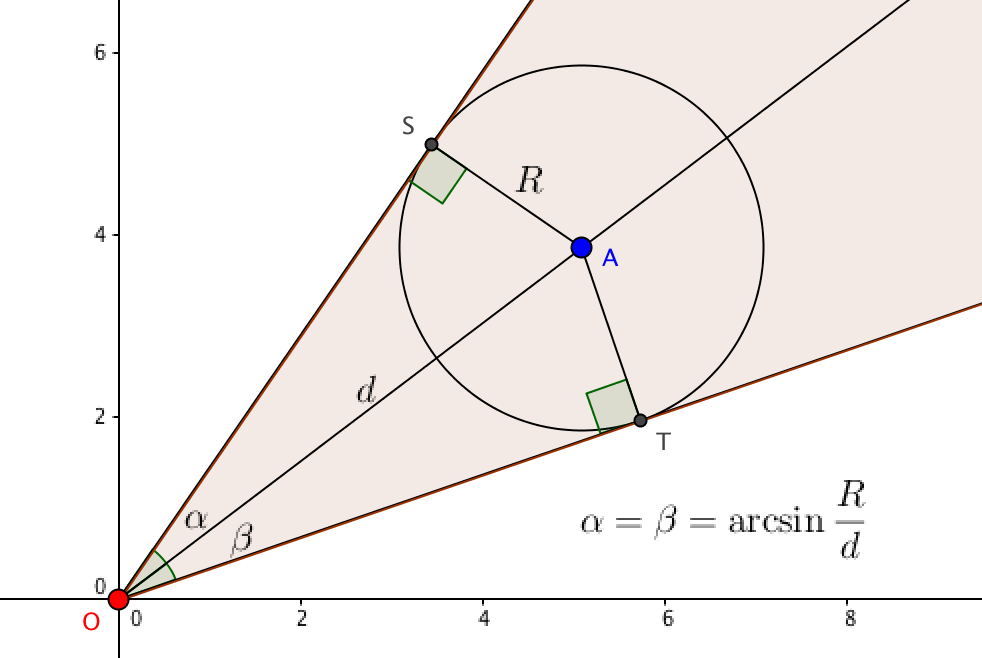
\includegraphics[scale=0.48]{a1.png}
\end{figure}

\end{frame}

\begin{frame}{Algorithm 2}

子任务 2:有滑条物件,物件影响的角度范围没有重叠部分。

\begin{figure}[h]\centering
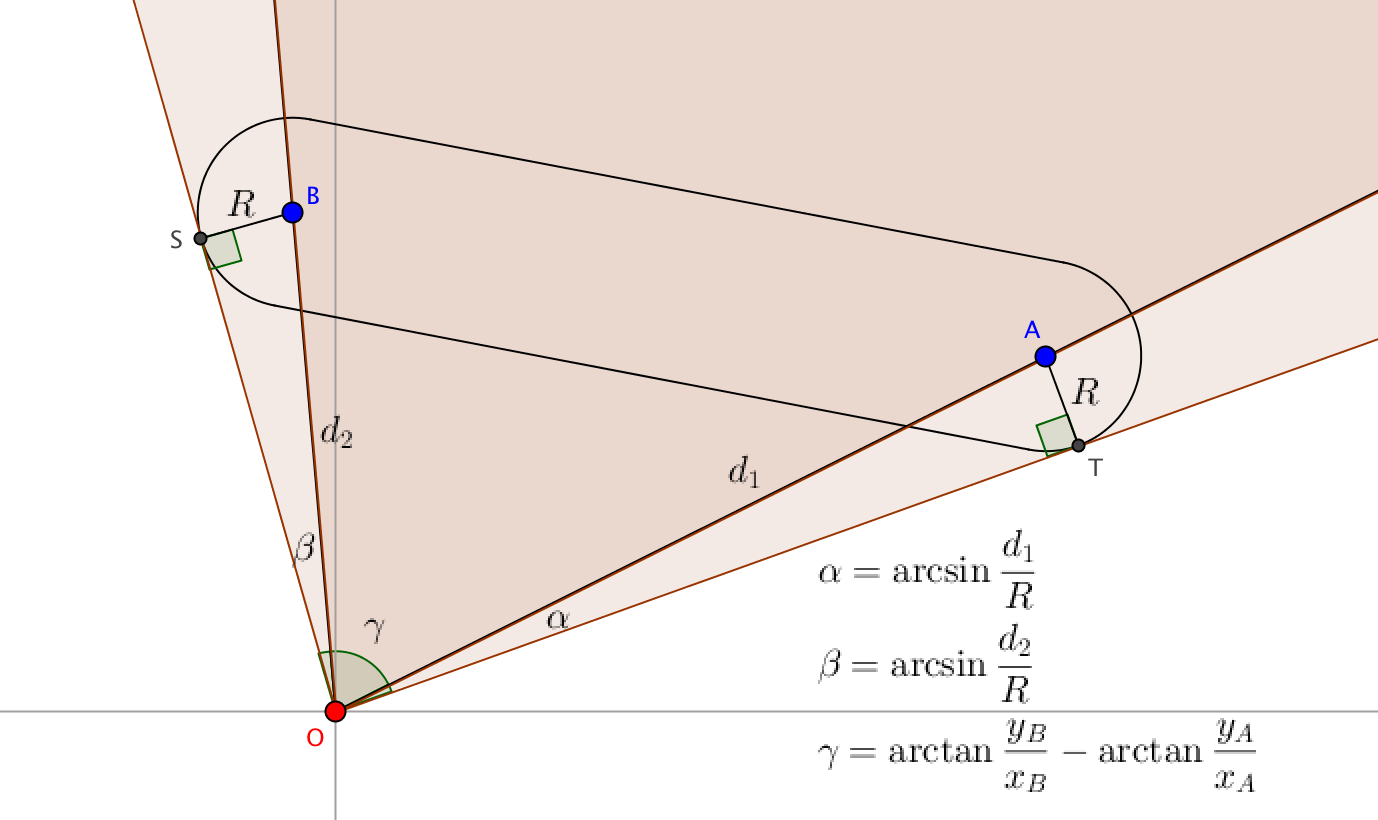
\includegraphics[scale=0.4]{a2.png}
\end{figure}

\end{frame}

\begin{frame}{Algorithm 2}

特殊情况:与上一种取 max

\begin{figure}[h]\centering
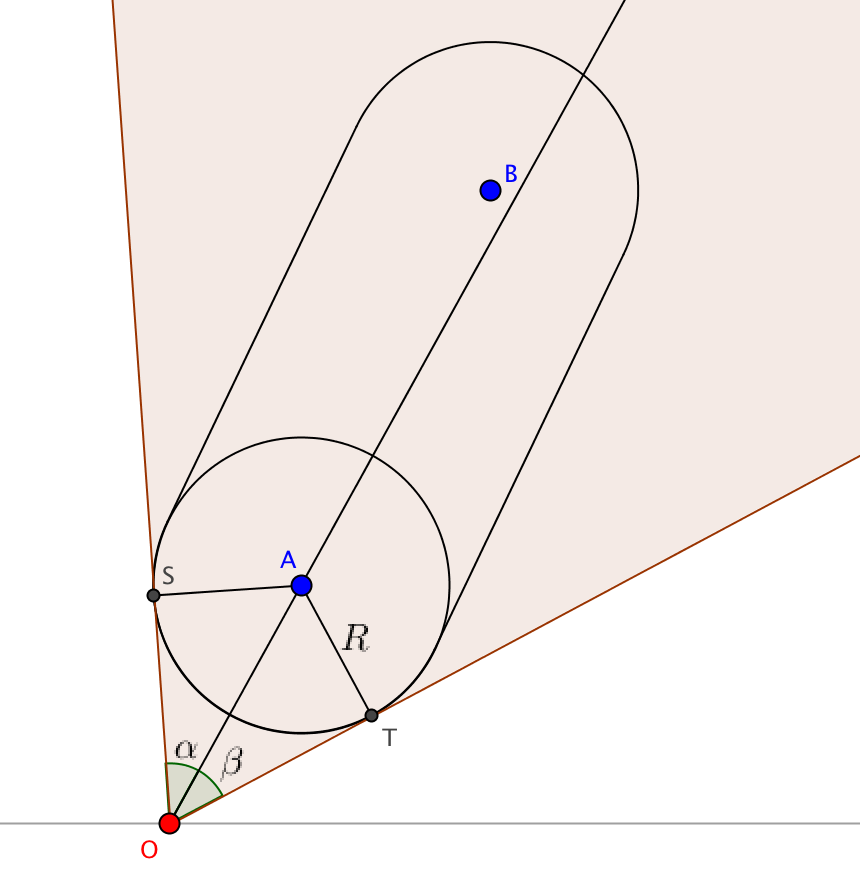
\includegraphics[scale=0.4]{a3.png}
\end{figure}

\end{frame}

\begin{frame}{Algorithm 3}

子任务 3:$N_\mathrm{C}, N_\mathrm{S} \leq 1\,000$ \newline

不会做,输出 QAQ

\begin{figure}[h]\centering

\includegraphics[scale=0.5]{xx.png}
\end{figure}

\end{frame}

\begin{frame}{Algorithm 4}

子任务 4:存在一条从原点出发的射线与每一个打击物件都有公共点。

\begin{figure}[h]\centering
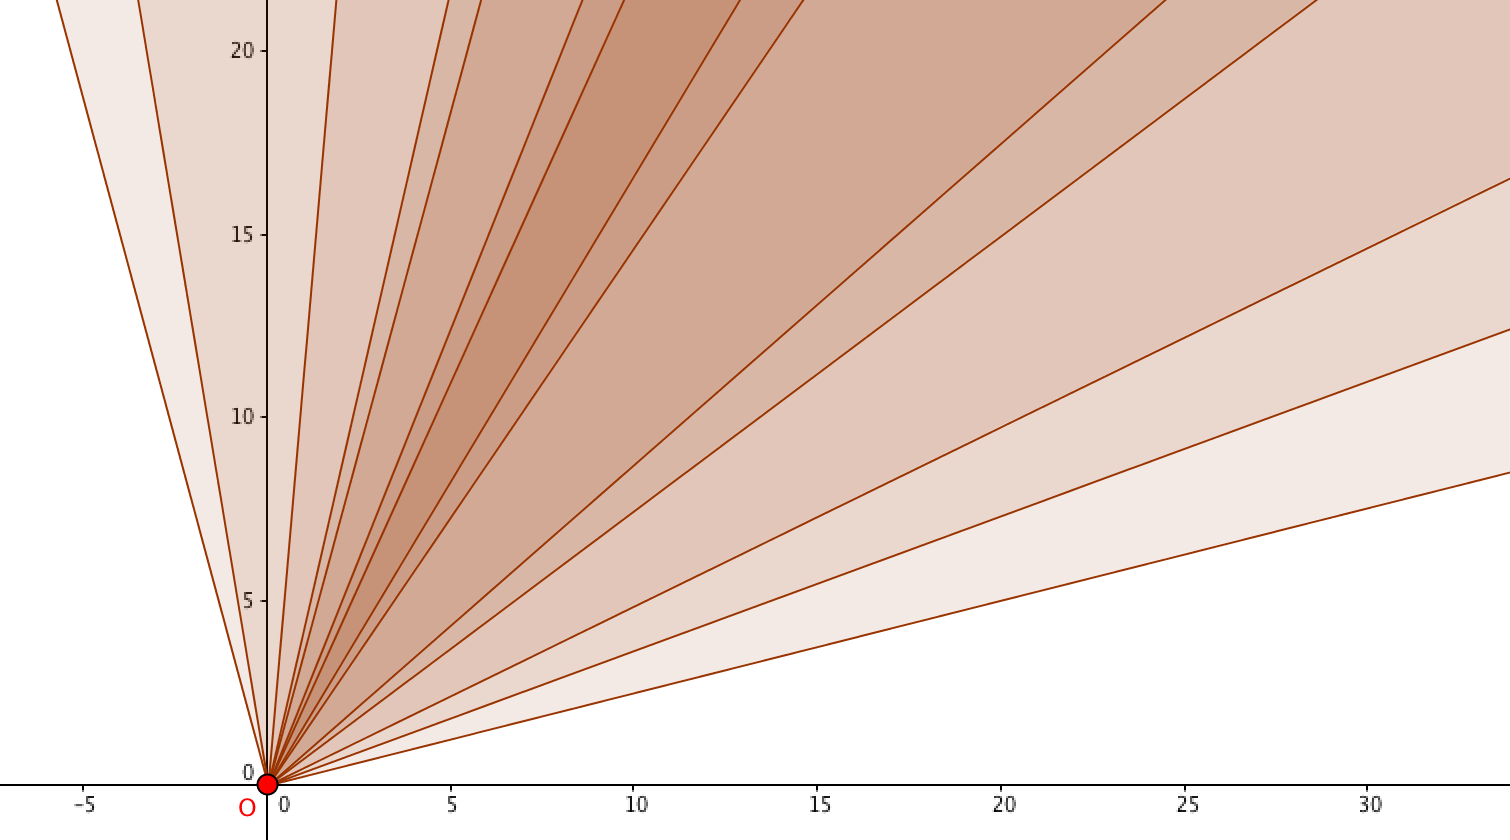
\includegraphics[scale=0.4]{a4.png}
\end{figure}



\end{frame}

\begin{frame}{Algorithm 5}

子任务 3:$N_\mathrm{C}, N_\mathrm{S} \leq 1\,000$ \newline

\begin{itemize}
    \pause \item 按照上述方法计算出每个物件影响角度的区间,记录端点(线?←\_←)并排序
    \pause \item 跨过 $\pm \pi$ 的位置拆分为两个区间
    \pause \item 枚举两个相邻端点,检查它们所夹区间是否被恰好一个物件覆盖
    \pause \item 排序 $O(N^2)$,枚举共 $O(N)$ 个区间,检查一次 $O(N)$
    \item 总时间复杂度 $O(N^2)$
\end{itemize}

\end{frame}

\begin{frame}{Algorithm 6}

我会快速排序!
\includegraphics[scale=0.666]{yy.png} \newline\newline

\pause $O(N \log N) + O(N^2) = O(N^2)$

\end{frame}

\begin{frame}{Algorithm 7}

“枚举两个相邻端点,检查它们所夹区间是否被恰好一个物件覆盖”\newline\newline

优化?

\end{frame}

\begin{frame}{Algorithm 7}

\begin{figure}[h]\centering
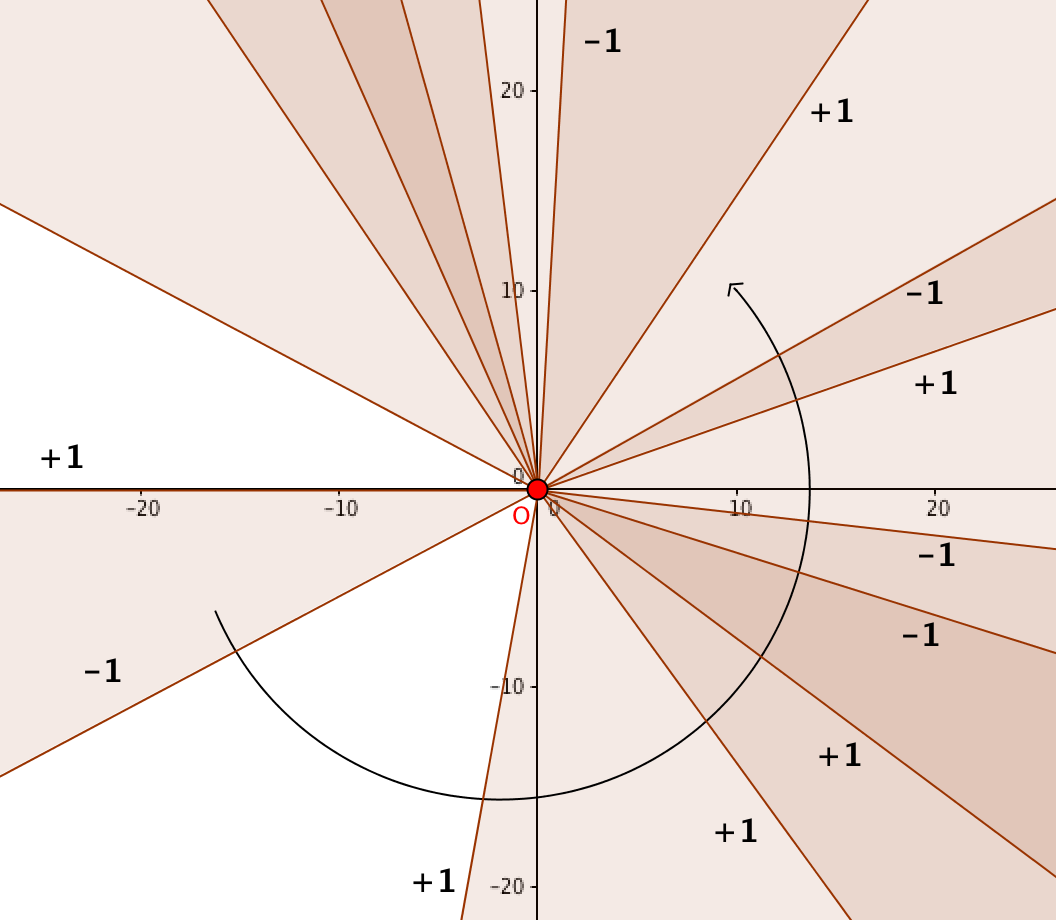
\includegraphics[scale=0.333]{a5.png}
\end{figure}

把区间转化成“事件”,对事件排序并依次处理,记录上个事件的位置与%
当前覆盖层数,判断层数 = 1 时增加答案。(常用 trick)

时间复杂度 $O(N \log N) + O(N) = O(N \log N)$

\end{frame}


\begin{frame}{Problem 2. OBSESSED}

给定一个序列,每个位置上为“空”、“面”音符与“边”音符中的一种。

进行下列操作:
\begin{itemize}
    \item 放置“面”或“边”音符;
    \item 询问一段连续区间内最近一对相同音符(“面”或“边”)之间的最小距离。
\end{itemize}

$N, M \leq 300\,000$

\end{frame}

\begin{frame}{Algorithm 1}

子任务 1、2:$N \cdot M \leq 600\,000$

直接模拟即可。注意反转操作的判定\newline\newline

\begin{algorithm}[H]
\begin{algorithmic}[1]
    \IF {$A[i] == \mathrm{DON}$}
        \STATE $A[i] := \mathrm{KAT}$
    \ELSE \STATE $A[i] := \mathrm{DON}$
    \ENDIF
\end{algorithmic}
\caption{ 
\includegraphics[scale=0.2]{zz.jpg}}
\label{alg:seq}
\end{algorithm}

\end{frame}

\begin{frame}{Algorithm 2}

子任务 3:没有“边”音符和反转操作,放置音符的位置严格单调递增

????

\end{frame}

\end{document}

